\section{Box dimension and \texorpdfstring{$D=1/H$}{D = 1/H}}\label{sec:dimension}

Do the flights and the crests share one geometry? $\Hroute$ is close to $\Hgeo$ (Section~\ref{sec:flights}), which reads as: the route is about as
straight as the crests. Both exponents come from a mean square displacement, so both depend on how a curve is parametrized and on which curves enter the mean.
Box counting measures the geometry with no parametrization and no mean square displacement. If a curve is self-similar and its parameter is the arc
length, its box dimension is $D=1/H$, so $D_{\mathrm{crests}}=1/\Hroute$ is a test that does not use the quantity it checks. We make two comparisons.
First, $D_{\mathrm{crests}}$ against $1/\Hgeo$ of the same paths: if they agree, the arc-length TAMSD of Section~\ref{sec:tamsd} measures the geometry.
Second, $D_{\mathrm{crests}}$ against $1/\Hroute$ of the flights. Agreement would mean that the route has the geometry of the crests;
$D_{\mathrm{crests}}<1/\Hroute$ that the route is rougher than the crest it follows, so the pilot adds structure; $D_{\mathrm{crests}}>1/\Hroute$ that it is straighter, so the pilot cuts corners.

\subsection{Theory}

For a fractional Brownian motion $B_H$ the graph of one component has dimension $2-H$ and the trace of the planar curve has dimension $\min(2,1/H)$. Any $H$-H\"older curve has dimension
at most $1/H$ (Falconer~\cite{falconer}); for fractional Brownian motion equality holds almost surely (Kahane, chapter~18~\cite{kahane}). Equality is not specific to fractional Brownian
motion. It holds for a self-similar curve whose parameter is proportional to its length at the resolution used: Brownian motion has $D=2$, the self-avoiding walk $D=1/\nu$
(de Gennes~\cite{degennes}), and the stable L\'evy processes have it with their self-similarity index in place of the MSD exponent. So agreement does not make the route a fractional Brownian motion,
which would need Gaussian stationary increments with its covariance.

The argument is short. A curve of length $\ell$ cut into pieces of arc length $s$ has $\ell/s$ pieces. A piece of arc length $s$ has diameter of the order of the chord $\sqrt{\mathrm{MSD}(s)}\propto s^{H}$.
With boxes of side $\varepsilon$ and $s(\varepsilon)$ defined by $\sqrt{\mathrm{MSD}(s(\varepsilon))}=\varepsilon$,
\begin{equation}
  N(\varepsilon)\simeq \frac{\ell}{s(\varepsilon)},\qquad
  D(\varepsilon)=-\frac{\mathrm d\ln N}{\mathrm d\ln\varepsilon}=\frac{\mathrm d\ln s}{\mathrm d\ln\varepsilon}=\frac{1}{\alpha(s(\varepsilon))},\qquad
  \alpha(s)=\frac12\frac{\mathrm d\ln\mathrm{MSD}}{\mathrm d\ln s}.
  \label{eq:dimalpha}
\end{equation}
The last step uses the local slope $\alpha(s)$ of Section~\ref{sec:tamsd}: $D(\varepsilon)=1/\alpha$ holds scale by scale, and $D=1/H$ where $\alpha$ is constant. The parameter must be the arc length.
A subordinated curve $X(t)=R(S(t))$ has the trace and the dimension of $R$ and another exponent in time, which is why $D$ is compared with $\Hroute$, the exponent along the arc length, and not with $\Hdyn$.

\subsection{Method}

\paragraph{Box counting.} For a curve sampled every \DmStep~m, $N(\varepsilon)$ is the number of squares of a grid of side $\varepsilon$ that hold a sample, averaged over \DmOffsets{} random shifts of the grid.
The box sizes are log-spaced, \DmPerDecade{} per decade, from \DmEpsMin~m (twice the 100~m cut-off of the smoothing) to \DmEpsMaxKm~km. For a straight line $N(\varepsilon)=a/\varepsilon+1$, since the two ends
add one box, so we fit $N-1$ for every curve.

\paragraph{Divider.} The curve is walked with a compass of opening $\varepsilon$, from each end, and $L(\varepsilon)$ is the length of the walk, including the last chord. Then $L\propto\varepsilon^{1-D}$ and
$D=1-\mathrm d\ln L/\mathrm d\ln\varepsilon$. The two estimators have different systematic errors, and their spread measures them.

\paragraph{The same curves for $D$ and $1/H$.} Curves are pooled in classes of length, so that the same curves are used at every box size of a class, and each window of arc length $s$ of Table~\ref{tab:hgeo} is
translated into box sizes by the chord. $D$ and $1/H$ are computed on the same curves and the same range of scales, with 95\% bootstrap intervals over whole trees for the crests and whole flights for the routes.
Appendix~\ref{app:dimension} gives the classes, the windows and the data.

\subsection{One dimension per group}

Table~\ref{tab:dim} gives, for each group and two windows of arc length, the box dimension $D_{\mathrm{box}}$, the divider dimension $D_{\mathrm{div}}$, $1/H$ on the same curves and range, and their differences.
The window from 0.1~km is the single fit per group, on boxes of \DmEpsMin~m to \DmCrAlpsFromEpsHiKm~km. The last window of Table~\ref{tab:hgeo} (beyond 10~km) is missing: it starts at boxes of about 7~km, which
need paths of 60~km and more, and \DmPoolAlpsGroups{} trees in the Alps and \DmPoolPyrGroups{} in the Pyrenees have them. The window from 0.1 to 1~km is in Appendix~\ref{app:dimension}.

\begin{table}[H]
\centering
\caption{On the crests and on the routes $D_{\mathrm{box}}$ equals $1/H$ within 0.01. Box dimension, divider dimension and $1/H$ of the same curves on the same range of box sizes; the differences
$D-1/H$ have 95\% bootstrap intervals. The routes are those of the paragliding flights of the same massif.}
\label{tab:dim}
\small
\setlength{\tabcolsep}{4pt}
\begin{tabular}{lccccc}
\toprule
window of $s$ & $D_{\mathrm{box}}$ & $D_{\mathrm{div}}$ & $1/H$ & $D_{\mathrm{box}}-1/H$ & $D_{\mathrm{div}}-1/H$ \\
\midrule
\textit{Alps crests} & & & & & \\
from 0.1~km & 1.051 & 1.065 & 1.059 & \ensuremath{-}0.008 (\ensuremath{-}0.010, \ensuremath{-}0.005) & 0.006 (0.005, 0.008) \\
1--10~km & 1.073 & 1.086 & 1.075 & \ensuremath{-}0.002 (\ensuremath{-}0.008, 0.005) & 0.011 (0.008, 0.015) \\
\midrule
\textit{Pyrenees crests} & & & & & \\
from 0.1~km & 1.054 & 1.070 & 1.064 & \ensuremath{-}0.010 (\ensuremath{-}0.015, \ensuremath{-}0.005) & 0.005 (0.004, 0.007) \\
1--10~km & 1.083 & 1.089 & 1.084 & 0.000 (\ensuremath{-}0.011, 0.010) & 0.006 (0.001, 0.011) \\
\midrule
\textit{Alps routes} & & & & & \\
from 0.1~km & 1.075 & 1.098 & 1.073 & 0.001 (0.001, 0.002) & 0.024 (0.024, 0.024) \\
1--10~km & 1.080 & 1.107 & 1.083 & \ensuremath{-}0.002 (\ensuremath{-}0.003, \ensuremath{-}0.002) & 0.024 (0.023, 0.025) \\
\midrule
\textit{Pyrenees routes} & & & & & \\
from 0.1~km & 1.088 & 1.111 & 1.081 & 0.006 (0.004, 0.008) & 0.030 (0.028, 0.032) \\
1--10~km & 1.098 & 1.131 & 1.096 & 0.002 (\ensuremath{-}0.001, 0.005) & 0.035 (0.032, 0.038)
\\
\bottomrule
\end{tabular}
\end{table}

The box dimension equals $1/H$ within 0.01, and the divider does on the crests (\DmCrAlpsFromDiffDiv{} in the Alps, \DmCrPyrFromDiffDiv{} in the Pyrenees). On the routes the divider is above $1/H$ by
\DmRtAlpsFromDiffDiv{} and \DmRtPyrFromDiffDiv. The two estimators differ from each other by \DmEstSpread{} on the crests and \DmEstSpreadRoute{} on the routes (Alps, window from 0.1~km), and the correction of the end box
is of the same order. These are the systematic errors, larger than the bootstrap intervals.

\subsection{Crests against routes}

Table~\ref{tab:dimcross} is the test of the question: the box and divider dimensions of the crests against $1/\Hroute$ on the same boxes.

\begin{table}[H]
\centering
\caption{The route is rougher than the crest below 1~km and as rough above. Dimension of the crests against $1/\Hroute$ of the routes of the paragliding flights of the same massif, on the same box sizes and class of curves. The differences
use independent bootstrap resamples of trees and flights, and have 95\% intervals.}
\label{tab:dimcross}
\small
\setlength{\tabcolsep}{4pt}
\begin{tabular}{lccccc}
\toprule
window of $s$ & $1/\Hroute$ & $D_{\mathrm{box}}$ & $D_{\mathrm{box}}-1/\Hroute$ & $D_{\mathrm{div}}$ & $D_{\mathrm{div}}-1/\Hroute$ \\
\midrule
\textit{Alps} & & & & & \\
from 0.1~km & 1.075 & 1.051 & \ensuremath{-}0.024 (\ensuremath{-}0.027, \ensuremath{-}0.022) & 1.065 & \ensuremath{-}0.010 (\ensuremath{-}0.013, \ensuremath{-}0.008) \\
0.1--1~km & 1.071 & 1.034 & \ensuremath{-}0.037 (\ensuremath{-}0.039, \ensuremath{-}0.035) & 1.051 & \ensuremath{-}0.021 (\ensuremath{-}0.022, \ensuremath{-}0.019) \\
1--10~km & 1.085 & 1.073 & \ensuremath{-}0.012 (\ensuremath{-}0.019, \ensuremath{-}0.004) & 1.086 & 0.001 (\ensuremath{-}0.004, 0.006) \\
\midrule
\textit{Pyrenees} & & & & & \\
from 0.1~km & 1.083 & 1.054 & \ensuremath{-}0.028 (\ensuremath{-}0.034, \ensuremath{-}0.022) & 1.070 & \ensuremath{-}0.013 (\ensuremath{-}0.018, \ensuremath{-}0.008) \\
0.1--1~km & 1.071 & 1.035 & \ensuremath{-}0.036 (\ensuremath{-}0.039, \ensuremath{-}0.033) & 1.052 & \ensuremath{-}0.019 (\ensuremath{-}0.022, \ensuremath{-}0.016) \\
1--10~km & 1.097 & 1.083 & \ensuremath{-}0.014 (\ensuremath{-}0.024, \ensuremath{-}0.003) & 1.089 & \ensuremath{-}0.008 (\ensuremath{-}0.016, 0.001)
\\
\bottomrule
\end{tabular}
\end{table}

The gap sits below 1~km, where $D_{\mathrm{crests}}-1/\Hroute$ is \DmXAlpsShortBox{} by boxes in the Alps, and it closes above 1~km (\DmXAlpsMidBox{} by boxes, \DmXAlpsMidDiv{} by the divider). The gap is already in $1/H$ alone, so it does not come from box counting.

The windows of $1/H$ of Table~\ref{tab:hgeo}, fitted on all the curves at each lag, would show the routes smoother than the crests in the window from 0.1~km, because each lag mixes populations of different lengths.
The dimension needs a fixed population, so the values of Table~\ref{tab:dimcross} are the ones to compare (Appendix~\ref{app:dimension}).

\subsection{Scale by scale}

Equation~\eqref{eq:dimalpha} gives $D(\varepsilon)=1/\alpha(s(\varepsilon))$ at every scale. Figure~\ref{fig:dimscales} compares the two for the class of at least \DmCrAlpsFromClassKm~km.

\begin{figure}
\centering
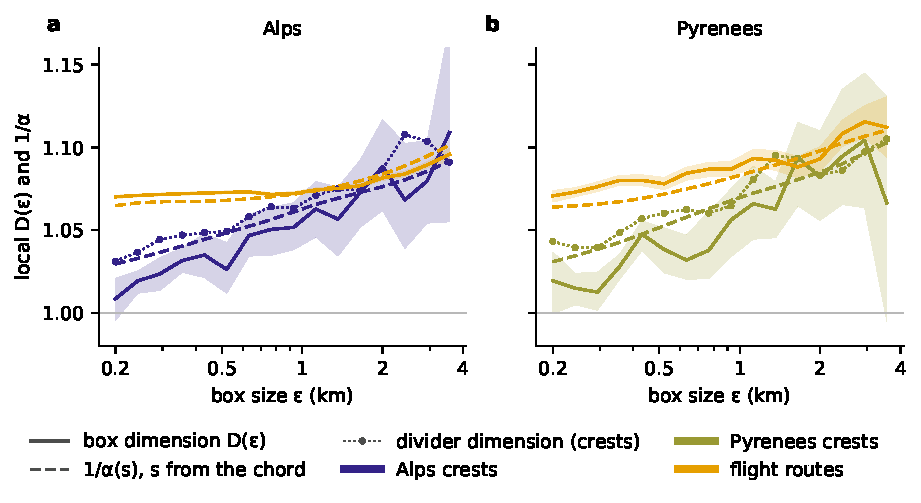
\includegraphics[width=\textwidth]{figures/dimension_scales.pdf}
\caption{On the crests the local box dimension follows $1/\alpha$, and the routes join the crests above 1~km. Local box dimension $D(\varepsilon)$ (solid, with the 95\% bootstrap band) and $1/\alpha(s)$ at $\sqrt{\mathrm{MSD}(s)}=\varepsilon$ (dashed)
for the crest paths of the massif (colour of the massif) and for the routes of the paragliding flights (orange), curves of at least \DmCrAlpsFromClassKm~km. Dotted with dots: divider dimension of the crests.
\textbf{a}~Alps. \textbf{b}~Pyrenees.}
\label{fig:dimscales}
\end{figure}

On the crests $D(\varepsilon)$ follows $1/\alpha$ from \DmEpsMin~m to a few kilometres. In the Alps the box dimension rises from \DmLocAlpsCrBoxLo{} at \DmEpsMin~m to \DmLocAlpsCrBoxHi{} at the top of the class.
The routes start higher and join the crests above 1~km. The last points of the crests have wide bands, and the Pyrenees show the same picture.

\subsection{What we keep}

On the crests $D=1/H$ holds by box counting within 0.01, and by the divider within about 0.01, on boxes of \DmEpsMin~m to \DmCrAlpsFromEpsHiKm~km. The routes satisfy it by box counting; their divider dimension is
higher by about 0.03. The range covers one decade, the dimension is close to 1, and the local dimension at \DmEpsMin~m is \DmLocAlpsCrBoxLo{} (box) in the Alps, where the smoothing at 100~m could be responsible.
We cannot separate $D\approx1.03$ from 1 at the lowest boxes, and on the rest of the range $D$ climbs with the scale, so the single value of a window depends on the range chosen.

Do the crests and the flights share one dimension? Above 1~km, yes within the method: the difference is within the spread between the estimators, about 0.02. Below 1~km, no: the route is rougher than the crest.
The pilot adds structure to the crest at the scale of a few hundred metres, and follows it above one kilometre. Beyond 10~km the data cannot say.
The joins do not lower $D$ (Appendix~\ref{app:dimension}), and the smoothing sets a floor at the lowest boxes that this elevation model cannot test. The single paths have the dimension of the main watershed of Fehr et al.~\cite{fehr}
and the network of the crests that of Rak et al.~\cite{rak} on the large boxes, and lower on the small ones.
